\subsection{(10\%) Cohen-Sutherland Clipping (2017 No. 3)}
A clipping window has the following geometry:
\begin{itemize}
    \item Window(left, right, bottom, top) = (200, 600, 100, 400)
\end{itemize}

A line with the following end points is drawn in the world:
\begin{itemize}
    \item[P1:] (650, 450)
    \item[P2:] (350, 300)
\end{itemize}

Show how the Cohen-Sutherland clipping algorithm will clip these lines and what their final endpoints, if any, are.  Show the coordinate values of P1 and P2 after each pass of the algorithm.

\rule{\textwidth}{0.1mm}

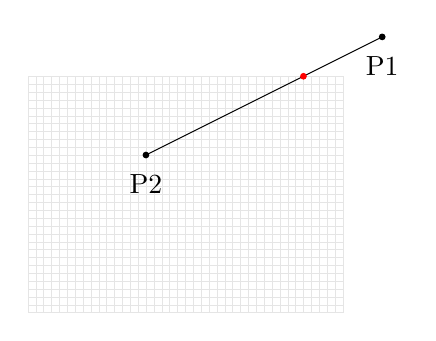
\begin{tikzpicture}[scale=0.1]
    \draw[step=1.0cm, gray!20, ultra thin](20, 10) grid (60, 40);
    \coordinate (P1) at (65, 45);
    \coordinate (P2) at (35, 30);
    \coordinate (C)  at (55, 40);

    \draw (P1) -- (P2);
    
    \filldraw (P1) circle (10pt) node[label={below:P1}]{};
    \filldraw (P2) circle (10pt) node[label={below:P2}]{};
    \filldraw[red] (C) circle (10pt);
\end{tikzpicture}

\begin{tabular}{|l|l|l|l|}
    \hline
    \verb|v \ >| & \textbf{left} & \textbf{center} & \textbf{right} \\ \hline
    \textbf{top}    & \verb|1010| & \verb|0010| & \verb|0110| \\ \hline
    \textbf{center} & \verb|1000| & \verb|0000| & \verb|0100| \\ \hline
    \textbf{bottom} & \verb|1001| & \verb|0001| & \verb|0101| \\ \hline
\end{tabular}

\begin{verbatim}
Iteration 0:
    // P1 = (650, 450)
    // P2 = (350, 300)

Iteration 1:
    // Bitmaks:
        code P1 = 0110
        code P2 = 0000
    
    P1 | P2 != 0000 -> Something is out of bounds
    P1 & P2 == 0 -> We need to clip
    
    // Clipping P1 from top:
        P1.x += (top - P1.y) * (P2.x - P1.x) / (P2.y - P1.y) // -100
        P1.y = 400
    
    // P1 = (550, 400)
    // P2 = (350, 300)

Iteration 2:
    // Bitmasks:
        code P1 = 0000
        code P2 = 0000

    P1 | P2 == 0 -> Both points are inside the window
    // -> The line gets drawn the final positions are:
    //      P1 = (550, 400)
    //      P2 = (350, 300)
\end{verbatim}